\documentclass{article}
\usepackage{hyperref} % used for links
\usepackage{listings}
\usepackage{circuitikz}
\usepackage{tikz}
\usepackage{xstring}
\usepackage{amsmath}
\usepackage{graphicx}
\usepackage{booktabs}

%--------------------Make usable space all of page
\setlength{\oddsidemargin}{0in}
\setlength{\evensidemargin}{0in}
\setlength{\topmargin}{0in}
\setlength{\headsep}{-.25in}
\setlength{\textwidth}{6.5in}
\setlength{\textheight}{8.5in}

\lstset{language=C, basicstyle=\ttfamily, breaklines=true}

% Hyperlink setup
\hypersetup{
colorlinks=true,
linkcolor=blue,
filecolor=magenta,
urlcolor=cyan,
}

% circuitikz shapes ---------------
%\makeatletter
% create the shape (switch without arrow) 
%\pgfcircdeclarebipole{}{\ctikzvalof{bipoles/interr/height 2}}{spst}{\ctikzvalof{bipoles/interr/height}}{\ctikzvalof{bipoles/interr/width}}{
%
%	\pgfsetlinewidth{\pgfkeysvalueof{/tikz/circuitikz/bipoles/thickness}\pgfstartlinewidth}
%
%	\pgfpathmoveto{\pgfpoint{\pgf@circ@res@left}{0pt}}
%	\pgfpathlineto{\pgfpoint{.6\pgf@circ@res@right}{\pgf@circ@res@up}}
%	\pgfusepath{draw}
%}

% make the shape accessible with nice syntax
% todo this breaks compilation
%\def\pgf@circ@spst@path#1{\pgf@circ@bipole@path{spst}{#1}}
%\tikzset{switch/.style = {\circuitikzbasekey, /tikz/to path=\pgf@circ@spst@path, l=#1}}
%\tikzset{spst/.style = {switch = #1}}
%\makeatother
% --------------------------------

% MATH -------------------------------------
% Vertical vector
\newcommand{\vvec}[1]{\begin{pmatrix}
                          #1
\end{pmatrix}}

\newcommand{\ipaddress}{http://192.168.8.42}

\begin{document}

    \tableofcontents
    \newpage

    \section{Maintenance}\label{sec:maintenance}
    NAS times are online for until around 14/9/2018.

    \subsection{Changing IP address}\label{subsec:changingIpAddress}

    To change IP address, change it in the Arduino code two times (\verb|myip| en \verb|gw|), if needed also change the NAS ip adress:
    \begin{lstlisting}
        ether.hisip[0]=192;
        ether.hisip[1]=168;
        ether.hisip[2]=178;
        ether.hisip[3]=29;
    \end{lstlisting}
    and the dns (directly under it).

    It may be needed to find the right dns for the NAS and the gw (gateway) address again, by doing a normal dhcp setup like
    \begin{lstlisting}
        ether.dhcpSetup();
        ether.printIp("IP: ", ether.myip);
        ether.printIp("GW: ", ether.gwip);
        ether.printIp("DNS: ", ether.dnsip);
        ether.printIp("SRV: ", ether.hisip);
    \end{lstlisting}
    Do not change the dns for the NTP server, \verb|dns[] = {195,121,1,34}|, otherwise the NTP dns lookup fails.

    Also change it in the Android app two times (\verb|ipString| and \verb|host|), and in the desktop app.

    The current ip address is \url{\ipaddress}.

    \subsection{Panels are stuck when out of bounds}\label{subsec:outOfBounds}

    For safety, when panels go out of bounds they cannot move anymore in any direction.
    To get them moving again, shortcut the low end stop if the panels are down like in Figure~\ref{lowendstop} and do the same for the high end stop if the panels are up like in Figure~\ref{highendstop}.


    \begin{figure}
        \centering
        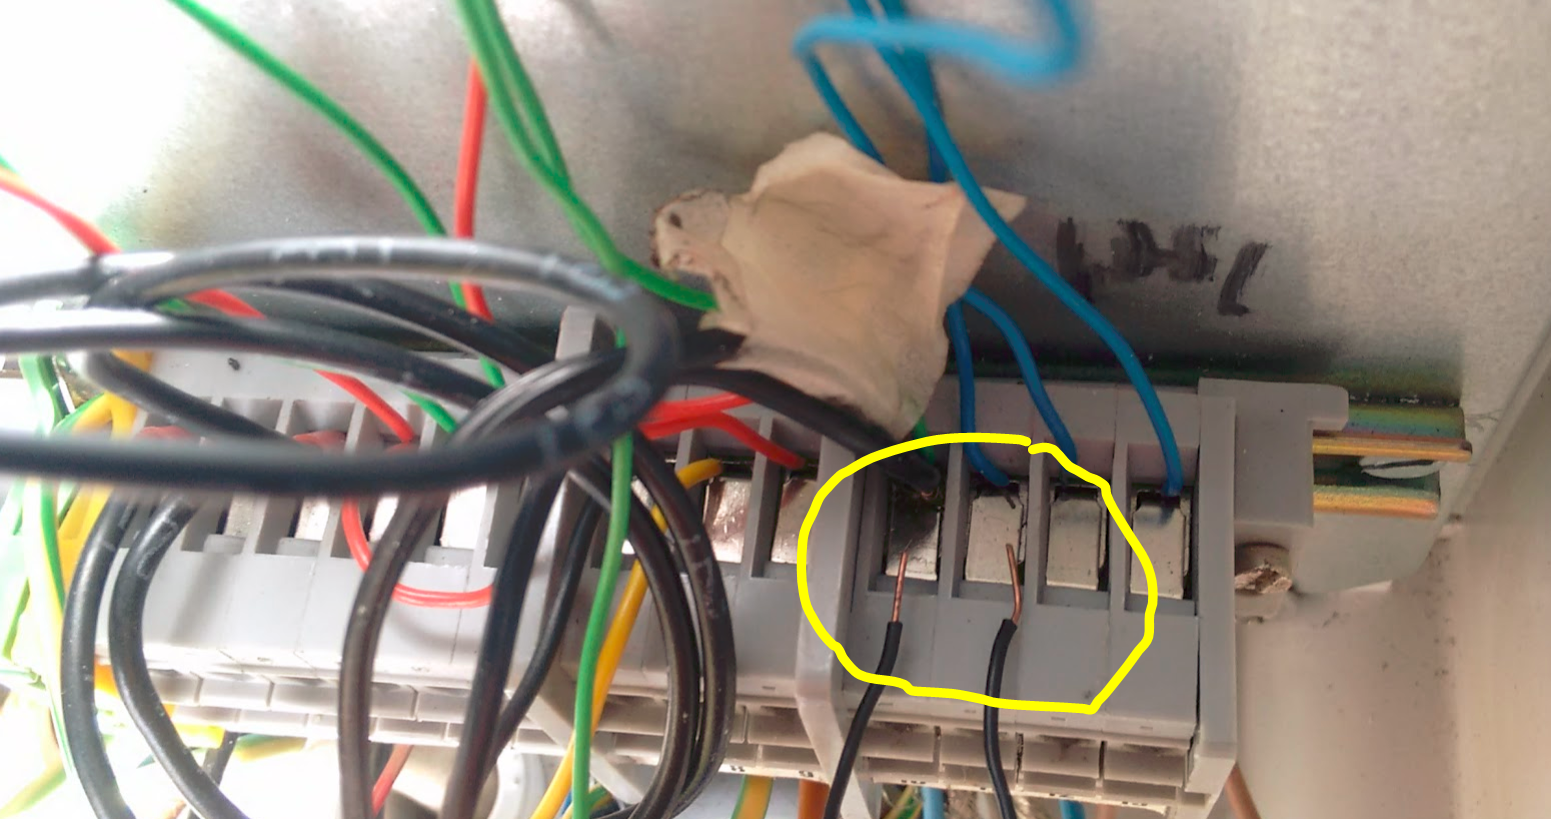
\includegraphics[width=.8\linewidth]{images/lowendstop.PNG}
        \caption{Shortcutting the low end stop}
        \label{lowendstop}
    \end{figure}
    \begin{figure}
        \centering
        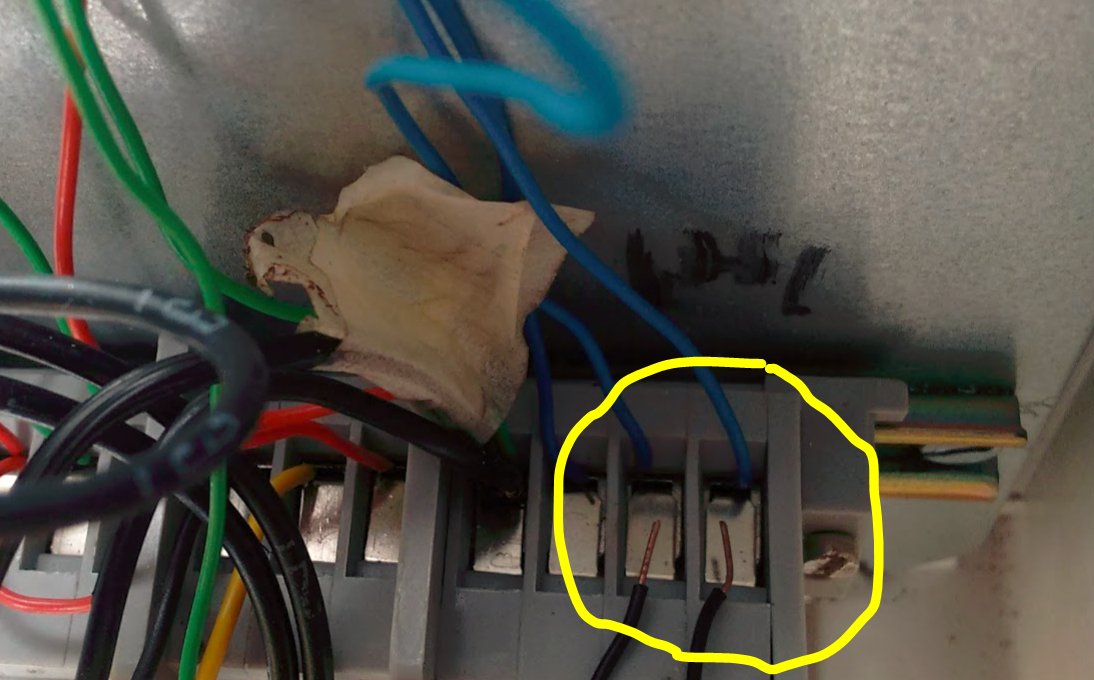
\includegraphics[width=.8\linewidth]{images/highendstop.PNG}
        \caption{Shortcutting the high end stop}
        \label{highendstop}
    \end{figure}

    \section{Setup of the project}\label{sec:setupOfTheProject}
    \subsection{Hardware used}\label{subsec:hardwareUsed}
We used an Arduino Nano ATmega328, bought at \href{http://nl.rs-online.com/}{rs-components}.
We used a \href{http://www.mijn-gadgets.nl/Webwinkel-Product-157562595/ENC28J60-Ethernet-Shield-Network-Module-V1.0-For-Arduino-Nano.html}{ENC28j60 Ethernet shield}, the version specifically for the nano.
This seemed easier than a wifi shield because of this reason, and with a wifi shield it seemed we needed extra components and a circuit, and we didn't really understand it.

Later when the NAS didn't want to process requests from the Arduino anymore, we bought a Micro SD Card Memory Shield Module from \url{https://www.gearbest.com/goods/pp_009462485053.html?wid=1433363&utm_source=email_sys&utm_medium=email&utm_campaign=shipping} and tried to get it to work with the ethernet shield, but that didn't work.

Then we bought a W5100 Micro SD Card Ethernet Shield from \url{https://www.gearbest.com/development-boards/pp_22810.html?wid=1433363}.
But we did not manage to get both the ethernet and the sd card to work.
Theoretically it should be possible, but in practice it seems like we want to let the Arduino do too much things together and it gets very difficult.
The test files can still be found in the UnitTests folder.

The best solution we could think of was buying a Raspberry Pi, see Section~\ref{ch:pi}.

\subsubsection{Components list}
	\begin{itemize}
		\item BC547 NPN transistor
		\item BC557 PNP transistor
		\item $4.7$k $\Omega$ resistor (yellow - violet - red - gold)
		\item $1$k $\Omega$ resistor (brown - black - black - brown - brown - red)
		\item $10$k $\Omega$ resistor (brown - black - orange - gold)
	\end{itemize}
\subsubsection{Button circuit}
	We implemented the begin- and endstops in the circuit for the buttons that move the panels up and down.
	When a button is NOT pushed, 1 and 1B, and 2 and 2B of that button are connected.
	When a button is pushed, connections are made between 1 and 1A, and 2 and 2A of that button.
	\begin{center}\begin{circuitikz}
		\draw 
		% 20, 28, E4
			(4,0) node {20} 
			(6,0) node {28}
			(8,0) node {E4}
		% button hoog
			(0.75 , -6) node {button up}
			(2.25, -5.25) node {1A}
			(2.25, -6) node {1}
			(2.25, -6.75) node {1B}
			(3.75, -5.25) node {2A}
			(3.75, -6) node {2}
			(3.75, -6.75) node {2B}
		% button laag
			(10 ,-6) node {button down}
			(7.25, -5.25) node {1A}
			(7.25,-6) node {1}
			(7.25, -6.75) node {1B}
			(8.5, -5.25) node {2A}
			(8.5, -6) node {2}
			(8.5, -6.75) node {2B}
		% drawing
			% 28 to 1,2 hoog via eindstoppen
				(6,-0.25) to (6,-1)
					to (3,-1) 
					to (3,-2)
				(2.5,-2) to (3.5,-2)
				(2.5,-2) to[switch, l_= high end stop] (2.5,-4) %eindstop hoog
					to (1.75,-4)
					to (1.75,-6) to (2,-6) 
				(3.5,-2) to[switch = low end stop] (3.5,-4) %eindstop laag
					to (4.25,-4)
					to (4.25,-6) to (4,-6) 
			% 1A hoog to 1B laag
				(2,-5.25) to (1.9,-5.25)
					to (1.9,-4.75)
					to(5.75,-4.75)
					to(5.75,-6.75)
					to(7,-6.75)
			% 2B hoog to 1A laag
				(4,-6.75) to (5.25,-6.75)
					to (5.25,-5.25)
					to (7,-5.25)
			% 20 to 1 laag
				(4,-0.25) to (4,-1.25)
					to (6.25,-1.25)
					to (6.25,-6)
					to (7,-6)
			% 1 laag to 2 laag
				(7.5,-6) to (8.25,-6)
			% E4 to 2A laag
				(8,-0.25) to (8,-4.75)
					to (9,-4.75)
					to (9,-5.25)
					to (8.75,-5.25)
		;
	\end{circuitikz}\end{center}
\subsubsection{Arduino circuit}
	\begin{center}\begin{circuitikz}
		\draw[dashed] 
			(2,10) to (5,10)
				to (5,14)
				to (2,14)
				to (2,10)
			(3.5,13) node[align=left] {Lenze\\ frequency\\ inverter}
		;
		\draw
		%E4 and its components (Arduino I/O, transistors)
			(10,0) node {E4}
			(1,1.225) node[align=center] {Arduino\\ I/O}
			(10,2) node [pnp] (pnpE4) {}
				(pnpE4.B) node[right=8mm, align=left] {Q6\\ BC557}
			(5,1.225) node [npn] (npnE4) {}
				(npnE4.B) node[right=8mm, align=left] {Q5\\ BC547}
		%Low end stop and its components
			(0.5,7.225) node[align=center] {Arduino\\ I/O}
			(10,8) node [pnp] (pnpLow) {}
				(pnpLow.B) node[right=8mm, align=left] {Q4\\ BC557}
			(4, 7.225) node [npn] (npnLow) {}
				(npnLow.B) node[right=8mm, align=left] {Q3\\ BC547}
		%High end stop and its components
			(0.5, 15.725) node[align=center] {Arduino\\ I/O}
			(10,16.5) node[pnp] (pnpHigh) {}
				(pnpHigh.B) node[right=8mm, align=left] {Q2\\ BC557}
			(4, 15.725) node[npn] (npnHigh) {}
				(npnHigh.B) node[right=8mm, align=left] {Q1\\ BC547}
		%Frequency Invertor and components (including line to GNDs)
			(3.5,11) node[sground] {}
				to (2,11)
			(1.2,11.5) node[align=left] {39 \\(GND)}
				(2,11) to[short,-*] (-1,11)
			(5.7,12) node[align=left] {28 \\ enable}
				(5,11.5) to (6.5,11.5) % fi to right
		%Arduino GND
			(-3,11) node[align=left] {Arduino\\ GND}
				(-2,11) to (-1,11)
				(-1,0) to (-1,14.955) % line on the left that connects GND
				(12,4) to (12,18.5) % line on the right that connects 20
		%circuit around E4
			(10,0.25) to (pnpE4.C)
			(pnpE4.B) to[R=R8 1k$\Omega$] (npnE4.C)
			(npnE4.E) to (5,0)
				to (-1,0)
			(npnE4.B) to[R, l=R7 4.8k$\Omega$] (2.1, 1.225)
			(9,2) node[circ] {}
				to[R,align=left, l=R9\\ 10k$\Omega$] (9,4)
				to (12,4)
			(10,4) node[circ] {} 
				to (pnpE4.E)
		%circuit around low end stop
			(pnpLow.B) to[R=R5 1k$\Omega$] (7,8) 
				to (npnLow.C)
			(9,8) node[circ] {} 
				to[R, align=left, l=R6\\ 10k$\Omega$] (9,10)
				to[short, -*] (12,10)
				(pnpLow.E) to (10,10) node[circ] {}
			(pnpLow.C) to[switch, align=left, l=low\\ end stop] (10,6)
				to (6.5,6)
				to (6.5,10) % up to high end stop
			(npnLow.B) to[R=R4 4.7k$\Omega$] (1.2, 7.225)
			(npnLow.E) to (4,6)
				to[short, -*] (-1,6)
		%circuit around high end stop
			(pnpHigh.B) to[R=R2 1k$\Omega$] (7,16.5)
				to (npnHigh.C)
			(9,16.5) to[R, align=left, l=R3\\ 10k$\Omega$, *-] (9,18.5)
				to (12,18.5)
			(pnpHigh.E) to[short, -*] (10,18.5)
			(pnpHigh.C) to (11.5,15.74) % from Q2 to right ...
			(11.5,15.74) to (11.5,7.225) % ... to right of Q4 ...
			(11.5,7.225) to[short,-*] (10,7.225) % ... to Q4
			(npnHigh.E) to (-1,14.955)
			(npnHigh.B) to[R=R1 4.7k$\Omega$] (1.2, 15.725)
			% draw end stop
			(6.5,11.5) to[switch, align=right, l=high end stop] (6.5,10)
		;
	\end{circuitikz}\end{center}
	\begin{tabular}{l|l|l|l}
		In circuit & terminal (connection to) & to meter cupboard & Arduino \\
		\hline
		Low end stop & no & white/green & 5 \\
		Ground & 4 & red/brown & GND \\
		E4 & 5 & blue & 4 \\
		High end stop & 6 & green & 3 \\
		\hline
		Circuit to potmeter &&& \\
		blue (signal) & 7 & black & A7\\
		yellow/green (+5V) & 8 & yellow & +5V \\
		brown (GND) & 9 & &
	\end{tabular}
\subsubsection{Potentiometer}
The \textbf{blue} wire from the potentiometer to the main control box is the signal wire, on connection 7 in that box.

Potmeter values as measured by the Arduino, scale 0--1024:

\begin{tabular}{ccc}
	Date & Low end stop & High end stop \\
	2017-10-22 & 360 & 74 \\
	2018-04-15 & 405 & 40 \\
\end{tabular}

\subsubsection{Motor control}
We bought BC547 NPN transistors to control the 12V/20mA (\href{http://download.lenze.com/TD/8201-8204__Inverter__v02-08__EN.pdf }{docs}, page 4--11) or 14V/40mA (measured) current of the EVF8202-E frequency inverter, and also base resistors otherwise the Arduino needs to give too much current to the transistor, and the transistor will be slow to turn off because of 'base charge storage'.

\subsection{Software used}\label{subsec:softwareUsed}

We have used the \href{http://platformio.org/platformio-ide}{PlatformIO IDE}, (which uses python 2.7 and Clang for autocompletion) because it is a lot better than the standard Arduino IDE, and also seemed better than the Stino plugin for Sublime Text 3.
A plugin for CLion also looked good but we didn't get that to work.
PlatformIO worked fine for a while but not always, so as a backup you can always use the Arduino IDE, but you need to copy all the libraries from \url{SolArduino_atom\\lib} to your \url{C:\\Users\\username\\Documents\\Arduino\\libraries} (Windows) or \url{~/Arduino/Libraries} (Linux) folder.
in the Arduino IDE you need to select the board (Arduino Nano) and select the ATmega328P (Old Bootloader), if you select the new bootloader it will not work.
This was last tested in the Arduino IDE 1.8.8.

    \section{Arduino Code}\label{sec:arduinoCode}
    \subsection{Internet/Ethernet connection}\label{subsec:internet/ethernetConnection}
    To connect the Arduino and the Ethernet shield to the internet, we used the \href{https://github.com/jcw/ethercard}{EtherCard} library.
    Because the ENC28j60 uses a different default CS pin (10 instead of 8), we had to add that in the code when making the connection.
    This is done by changing

    \begin{lstlisting}
    if (ether.begin(sizeof Ethernet::buffer, mymac) == 0)
    \end{lstlisting}

    (with no pin specified, so the default pin is used) to

    \begin{lstlisting}
    if (ether.begin(sizeof Ethernet::buffer, mymac, 10) == 0)
    \end{lstlisting}

    Note the third argument \lstinline|10| added after \lstinline|mymac|.
    To get the current time using NTP, we adapted \href{http://forum.arduino.cc/index.php?topic=171941.0}{example code} from the Arduino forum.

\subsection{Solar Panel control}\label{subsec:solarPanelControl}
    The calculation to find the goal value of the potmeter is within one voltage point accurate, which is because of the rounding to an integer voltage at the end.
    The calculation itself as implemented on the Arduino is 0 to 0.01 off, because of the rounding of the long value.
     The offset can be seen with this Mathematica command
    \begin{lstlisting}
    Plot[N[360 + ((x - 5)*100/(50 - 5))*(74 - 360)/100] -
    N[360 + Floor[((x - 5)/(50 - 5))*100*(74 - 360)]/100], {x, 10,
    10.01}]
    \end{lstlisting}
    which illustrates the difference between the exact solution and the Arduino code without rounding to the integer \verb|expectedVoltage|, which was implemented as
    \begin{lstlisting}
    float fraction = ( ( (float) ( (degrees - DEGREES_LOWEND) ) ) / (float) (DEGREES_HIGHEND - DEGREES_LOWEND) );
    int expectedVoltage = POTMETER_LOWEND +
    ( (long) ( fraction*100 * (POTMETER_HIGHEND - POTMETER_LOWEND) ) ) / 100 ;
    \end{lstlisting}
    The idea is to keep setting the right pins high until the difference between the current voltage and the expected voltage is zero.
    If the potmeter happens to skip the value, no problem occurs because the Arduino keeps no memory of that and will try to reach the right value again.
    Tests showed that with sufficient sampling of the input the value may in a rare situation be skipped once but not more.

\subsection{Storage of angles}\label{subsec:storageOfAngles}
    Because the Arduino program space could by far not store all the unix times and angles for like a year, we decided to use a webserver on the Synology NAS as storage space.
    Every time the Arduino runs out of angles, it detects that either in the \verb|loop()| or in \verb|solarPanelAuto()|, and then requests new angles at \url{http://192.168.2.7} with \verb|requestNewTable()|. After sending such a request, the program needs to wait for a response before continuing, otherwise it continues with old angles.
    The `waiting' is implemented with a global flag variable \verb|responseReceived|, which is set true in the callback after the angle and date arrays are updated.

    Currently the arrays are of size 10, and therefore the little PHP script on the NAS gives the next ten angles and dates when called.
    The number ten is chosen because of RAM limitations, if you want to change it, change the \verb|tableLength| global variable, the number in the declarations of the arrays, the number of times the PHP script gives back, the \verb|tableSize| which indicates how many bytes the NAS response will need, and is used in the ethernet buffer and when parsing.
    To calculate that size, given $x$ angles, you'd do something like $11x$ for the dates plus $4x$ for the angles and a little more plus about 140 bytes/characters from the http header would be around 300 bytes for 10 angles.
    But tests point out almost 400 bytes are needed here, so be sure to test it well.
    In the NAS, you can find the page with the file browser under \verb|DiskStation/web/index.php|.

\newcommand{\ipaddress}{http://192.168.8.42} % todo

\subsection{Communication with the Android app} \label{subsec:arduinotoandroid}
    \subsubsection{Request}
    Communication goes by http requests, in the form of \url{http://192.168.2.106/?key=value}.
    Currently implemented are the following parameter options.

    \begin{tabular}{ll}
        \verb|panel=up| & The panels will move up. \\
        \verb|panel=down| & The panels will move down. \\
        \verb|panel=stop| & The panels will stop moving.
        \verb|panel=auto| & The panels will go in automatic mode. \\
        \verb|degrees=x| & The panels will go to $x$ degrees. \\
    \end{tabular}

    \subsubsection{Result}
    The result will be in the form of % todo
    The result will always contain the current angle of the panels.

\subsection{Safety measures}\label{subsec:safetyMeasures}
    In order to avoid relying on the hardware end stops, a few safety measures were introduced:
    \begin{itemize}
        \item A soft bound was introduced for the potmeter constants and degrees constants.
        We hope this catches varying potmeter bounds: sometimes the value of the low end may be a few points lower and then the code would try endlessly to get the solar panels below their hardware end stop.
        \item In the \verb|solarPanelDown| and \verb|solarPanelUp| methods, as close to the solar panel control as possible, we put an extra check if the reading of the analog pin does not go out of bounds.
        These bounds therefore include the soft bounds.
        This check intentionally does not rely on \verb|readPotMeter()| (which samples readings for better accuracy), which reduces accuracy near the soft end stops but increases safety.
        Accuracy inbetween should not be influenced.
        Moreover, when there is an emergency the panels are stopped by the Arduino, ensured in the main loop.
        To be more precise: we assume the lowest number of the potmeter value corresponds to the lower end stop.
        In the code we check that when going down the potmeter value should be higher than the potmeter low end constant, therefore the panels cannot move down when below the (soft) end stop according to the potmeter.
        If the check fails, the internal EmergencyState is set to ``panels below lower bound!'', which can only be removed in solarPanelUp when the potmeterpin is above the low end constant and the EmergencyState contains exactly the mentioned sentence, or on a reboot of the Arduino.
        Therefore the panels cannot move downwards by Arduino signals when below the low end stop.
        For moving up of course everything is the other way around.
        \item The Arduino now has a timeout on moving the panels up or down, which means that when you do not send another up/down request within the timeout of $x$ seconds the panels will stop automatically.
        The app and desktop version now try to send a request each $\frac{x}{2}$ seconds, but subject to change.
        Especially because of the in practice noticed bad connections this is a very practical alternative to keeping an open connection which would be even better but is a bit complicated with an Arduino.
        \item The high and low end stop were put in series, such that \textit{all power} which can move the panels goes via \textit{both} end stops.
        That means that whatever happens, as long as the physical end stops work the panels will not go through their end stops anymore.
        This of course also means that when they do, by Arduino accident or (more probably) by manual buttons, you have to shortcut the end stop with an extra wire (just hold it to both connectors) to get it moving again (one can use the manual buttons).
    \end{itemize}

    \section{Raspberry Pi API} \label{subsec:arduinotoandroid}

    

Communication goes by http requests, in the form of \url{\ipaddress/?key=value}.

\subsection{Request}
Currently implemented are the following parameter options.

\begin{tabular}{ll}
    \verb|panel=up| & The panels will move up until a timeout is reached, or
    a new up or down request is sent. \\
    \verb|panel=down| & The panels will move down under the same conditions. \\
    \verb|panel=stop| & The panels will stop moving and disable automatic mode. \\
    \verb|panel=auto| & Enable automatic mode. \\
    \verb|panel=manual| & Disable automatic mode. \\
    \verb|degrees=x| & The panels will go to $x$ degrees. \\
    \verb|emergency=reset| & If the system is in emergency mode, the emergency will be reset. \\
\end{tabular}

\subsection{Response}

The result will be in the form of json, containing the following values.

\begin{tabular}{ll}
    \verb|emergency: boolean| & Whether the system is in emergency mode or not. \\
    \verb|angle: float| & Current angle of the panels. \\
    \verb|auto_mode: boolean| & Whether the system is in automatic mode. \\
    \verb|message: string| & Human readable response message containing more information about the response, or error message in case of emergency. \\
    \verb|min_angle: float| & Lowest angle the panels can be set at. \\
    \verb|max_angle: float| & Highest angle the panels can be set at. \\
\end{tabular}

\section{Android App User Manual}\label{subsec:userManual}
To move the solar panels up (or down), press the up (or down) button and hold it until the desired position/angle is reached.
The current degree on the top right and the picture updates while the button is held, so you know when the panels are at the desired position.

To set the solar panels in auto mode, press the auto checkbox.


To set the solar panels at a certain degree, move the slider until the $x$ at the button which says "\verb|SET ANGLE AT | $x^{\circ}$" is the desired degree for the angle.
Then press the button to set the angle of the panels at that degree.
May you change your mind about the angle while the panels are moving, stop the panels with the stop button at the bottom and send a new angle request.

To update the |TextView| containing the current angle, simply press the number.
This will also update the position of the picture.
This will also check the checkbox if the panels are in auto mode, and uncheck the checkbox if the panels are not in auto mode (if needed).


    \section{Calculations}\label{sec:calculations}
    \subsection{Finding the angle between the sun and the line perpendicular to the solar panels}\label{subsec:findingTheAngleBetweenTheSunAndTheLinePerpendicularToTheSolarPanels}
To find the angle $\alpha$ between the sun and the line perpendicular to the solar panel, we determined both lines in spherical coordinates (with the same distance to the origin) and then calculated the angle between the two.


For the sun this would be
\[
    \vvec{x \\ y \\ z} =
    \vvec{\cos \gamma_s \sin \left(\frac{\pi}{2} - \theta_s\right) \\
    \sin \gamma_s \sin \left(\frac{\pi}{2} - \theta_s\right) \\
    \cos \left(\frac{\pi}{2} - \theta_s\right)}
\]
where $ \gamma_s $ is the azimuth, and $ \theta_s $ the altitude of the sun.


For the line perpendicular to the solar panels this would be
\[
    \vvec{x \\ y \\ z} =
    \vvec{\cos \gamma_p \sin \left(\frac{\pi}{2} - \theta_p\right) \\
    \sin \gamma_p \sin \left(\frac{\pi}{2} - \theta_p\right) \\
    \cos \left(\frac{\pi}{2} - \theta_p\right)}
\]
where $ \gamma_p $ is the azimuth (direction of the solar panels in respect to the South), and $ \theta_p $ the altitude of the solar panels.

Then, to find the angle $\alpha$ between these two lines, we take the $ \arccos $ of the dot product.
This gives us

\[
    \alpha = \arccos (\cos (\gamma_p - \gamma_s) \cos \theta_s \sin \theta_p + \sin \theta_s \cos \theta_p)\,.
\]

\subsection{Implementation of calculations to find optimal angles}

\subsubsection{Mathematica calculations}\label{subsec:mathematicaCalculations}

The Mathematica package (imported with \verb|<< SolArduino`|, be sure to place it in your
\url{\%AppData\%\\Mathematica\\Applications} folder) can calculate the optimal angle for a given day.
To do that, it calculates for each angle between $0$ and $90$ the total of the insolation (power received by the sun) at each half hour of that day.
Then it finds the angle for which that value is maximal.
To find the insolation at a given hour, the function \verb|angle| calculates the misalignment with the sun using the formula from the previous subsection, and then calculates the insolation using a formula from \href{http://www.powerfromthesun.net/Book/chapter02/chapter02.html#ZEqnNum929295 }{www.powerfromthesun.net}, where parameters for urban haze compared a lot better with real life values (17/8) than clear day parameters.

It can therefore make graphs for optimal angles for a month, and averaging the values for a month, also for a year, and lots more as seen in the demonstration notebook.
When plotting real data, for example days like 13/5, 19/7 and 17/8 are all cloudless days with the solar panels at around 25 degrees.

It is important to note that the functions \verb|angle|, \verb|directPower| and more do not take the hour of the day as input, but the index of the \verb|sunPositions| table which contains the azimuth and altitude of the sun over the day.
Therefore, \textit{before you call functions which take an index as parameter you need to make sure you have }\verb|sunPositions| \textit{initialised} at the right day, done by calling \verb|calculatesunPos[DateObject[{2016,7,18}]]| with whatever day you want in the table.

Exporting the angles for ten times a day for two years, like

\verb|exportPeriod[DateObject[{2016, 9, 7}], DateObject[{2018, 9, 15}], 10]| took only ten minutes (Lenovo W541 laptop on high performance).

\subsubsection{Haskell calculations}

Because Mathematica is proprietary, we decided to also provide a Haskell implementation.
It uses the \href{https://hackage.haskell.org/package/astro}{Astro package} to find the position of the sun.

    \section{Raspberry Pi}\label{ch:pi}
    As explained in Section~\ref{subsec:hardwareUsed} when the NAS stopped serving requests we decided to drop the Arduino and start using a Raspberry Pi.

There are a lot of Raspberry Pi versions, but at the moment of writing (March 2019) it seems the Raspberry Pi 3 B+ is the most recent and complete Pi.
However, since a Raspberry Pi has no analog inputs, we will need a separate Analog to Digital Converter (ADC) to read the pot meter values.
It seems that the MCP3008 is widely used, see for example \url{https://electronicshobbyists.com/raspberry-pi-analog-sensing-mcp3008-raspberry-pi-interfacing/}.
It speaks about setting 3.3v on the potmeter, just like all other places we could find, whereas we put 5v on it with the Arduino but we think it should work all the same.


\end{document}